\documentclass[stage2a]{tnreport}


\usepackage{dsfont}
\usepackage{glossaries}
\usepackage{enumitem}

\def\reportTitle{Analyse exploratoire des données spatialisées en utilisant des processus ponctuels} % Titre du mémoire
\def\reportLongTitle{Analyse exploratoire des données spatialisées en utilisant des processus ponctuels} % Titre plus long du mémoire

\def\reportAuthor{Clément Dugué}
\def\reportAuthorEmail{\email{clement.dugue@telecomnancy.net}}

\def\reportAuthorAddress{46 rue de Laxou}
\def\reportAuthorCity{54000, NANCY}
\def\reportAuthorPhone{06 11 68 21 32} 

\def\reportIndustrialSupervisor{Radu STOICA}
\def\reportAcademicSupervisor{Sébastien DA SILVA}

\def\reportCompany{Institut Elie Cartan de Lorraine}
\def\reportCompanyAddress{Campus Sciences BP 70239}
\def\reportCompanyCity{54506, VANDOEUVRE LES NANCY}
\def\reportCompanyPhone{03 72 74 54 19}
\def\reportCompanyLogoPath{figures/iecl.png} 

\def\place{Nancy}
\def\date{\today}



\makeglossaries
\newglossaryentry{PP}
{
    name=processus ponctuels,
    description={Type particulier de processus stochastique pour lequel une réalisation est un ensemble de points isolés du temps et/ou de l'espace. Par exemple, la position des arbres dans une forêt peut être modélisée comme la réalisation d'un processus ponctuel}
}

\newglossaryentry{PPoiss}
{
    name=processus de Poisson,
    description={Nommé d'après le mathématicien français Siméon Denis Poisson et la loi du même nom, est un processus de comptage classique dont l'équivalent discret est la somme d'un processus de Bernoulli. C'est le plus simple et le plus utilisé des processus modélisant une file d'attente. C'est un processus de Markov, et même le plus simple des processus de naissance et de mort.}
}

\newglossaryentry{PPPoiss}
{
    name=processus ponctuel de Poisson,
    description={Le processus ponctuel de Poisson est le plus simple et le plus universel des \gls{PP}*. C'est une généralisation spatiale du \gls{PPoiss}* utilisé en théorie des files d'attentes}
}

\newglossaryentry{stationnaire}
{
    name=stationnaire,
    description={dont les propriété ne changent pas selon l'endroit où l'on regarde}
}

\newglossaryentry{statDescriptive}
{
    name=statistique descriptive,
    description={ technique utilisée pour décrire un ensemble relativement important de données}
}

\newglossaryentry{spatstat}
{
    name=librairie spatstat,
    description={ librairie fournissant des méthode de calcul pour l'étude de statistiques spatiales, spatstat est plutôt orienté vers les calculs en 2 Dimensions}
}

\newglossaryentry{double}
{
    name=double,
    description={ nombre codés sur 64 bits entre \begin{math}-1.7*10^{-308} \end{math} et \begin{math}1.7*10^{308}\end{math} }
}

\newglossaryentry{namespace}
{
    name=namespace,
    description={ lieu abstrait conçu pour accueillir des ensembles de termes appartenant à un même répertoire}
}

\begin{document}
  
\maketitle
\pagenumbering{roman}

\insertAntiPlagiarismAgreement{Dugué, Clément}{2406037702x}

\cleardoublepage

\makesecondtitle

\section*{Remerciements}
\addcontentsline{toc}{chapter}{Remerciements}

{\em
En premier lieu, je tiens à remercier la direction de l'institut Elie Cartan et M. Xavier ANTOINE responsable de l'équipe de Probabilités Statistiques pour m'avoir accueilli dans le laboratoire.\\

J'adresse également mes remerciements à mon maître de stage M. Radu STOICA pour ses explications, son soutien et son écoute tout au long du stage, ainsi que pour la confiance qu'il m'a accordé en m'acceptant comme stagiaire.\\

Je souhaite aussi remercier mon encadrant universitaire M. Sébastien DA SILVA qui a participé au bon déroulement de ce stage.\\

Je remercie enfin toutes les personnes m'ayant aidé dans l'écriture et la relecture de ce rapport de stage.
}

\cleardoublepage

\renewcommand{\baselinestretch}{0.5}\normalsize
\tableofcontents
\renewcommand{\baselinestretch}{1.0}\normalsize
\cleardoublepage

\pagenumbering{arabic}
\setcounter{page}{1}

\chapter{Introduction}


Lorsqu'on rassemble des données pour une étude (localisation d'évènements historiques, de micro-organismes, de populations...), il est pratique de représenter ces données sous forme de points. On obtient alors une répartition ponctuelle des données pouvant être analysée. On peut ainsi identifier des tendances selon la densité des points (si les points sont rapprochés ou non), c'est l'analyse statistique. Les résultats de l'analyse peuvent ensuite être interprétés pour en tirer des conclusions, et fournir ainsi des informations objectives utiles pour de nombreux domaines.

L'automatisation de cette analyse ce fait par la création de programme informatique qui peuvent lire les données fournies et faire des calculs rapides.
Cependant il n'y a pas de solution toute faite pour l'analyse statistique de répartition de points, en effet chaque cas doit être analysé en fonction de son contexte (obtention des données, objectif de l'analyse). D'où le besoin de fonction et de programmes multiple pour cette analyse.

Ce fut le but de ce stage: créer des outils informatique pour traiter et analyser des données ponctuelles selon des méthodes mathématiques fournies et expliquées par mon tuteur.
La réalisation des fonctions se faisait en plusieurs étapes: d'abords la lecture et compréhension de la documentation sur la fonction, puis la conception et l'écriture du code, et enfin une analyse des résultat obtenus en vus d'une amélioration (retour à la 2ème étape). Ainsi, après un présentation globale de l'entreprise d'accueil, la structure de ce rapport suivra cet enchaînement en regroupant pour chaque étapes toutes les fonctions réalisées. 

Enfin sachez que les références vers le glossaire seront indiquées par un * .

\newpage

\chapter{Présentation de l'entreprise d'accueil}

En attente de réponse au mail : copié collé de la page internet iecl

\section{Institut Elie Cartan}
Fondée il y a plus de cent ans, avec l’arrivée d’Élie Cartan comme professeur à la Faculté des Sciences de Nancy, la recherche lorraine en mathématiques a une longue tradition, marquée par une succession de personnalités de renommée mondiale comme Jean Leray, Laurent Schwartz (Médaille Fields 1950), Jean-Pierre Serre (Médaille Fields 1954), Roger Godement, Jean Delsarte (secrétaire du groupe Bourbaki jusqu’en 1962) ou Jacques-Louis Lions.

Créé en 1953 à l’initiative de Jean Delsarte, l’Institut Élie Cartan de Nancy a été reconnu par le CNRS en 1978 (sous le nom d’Équipe d’Analyse Globale) et il a fusionné avec le Laboratoire de Mathématiques et Applications de Metz au premier janvier 2013. Le nouveau laboratoire est intitulé Institut Elie Cartan de Lorraine (IECL),

\section{L'IECL}
L’IECL est une unité mixte de recherche (UMR 7502) du CNRS et de l’Université de Lorraine. L’INRIA est un partenaire important et de longue date de l’IECL, notamment à travers les équipes-projets INRIA que nous hébergeons.

Avec environ 120 enseignants-chercheurs et chercheurs permanents, l’Institut Élie Cartan de Lorraine est l’un des grands laboratoires français en mathématiques et le plus grand de l’Est de la France.

 Dans plusieurs domaines des mathématiques fondamentales (géométrie, théorie des nombres), des équations aux dérivées partielles ou des probabiliés, l’IECL rassemble des spécialistes reconnus internationalement. Cette diversité scientifique favorise les interactions internes et externes, en contribuant à l’attractivité pour les visiteurs étrangers.

\newpage

\section{L'equipe Probabilités et Statistiques}

L’équipe de Probabilités et Statistique est l’une des quatres équipes de l’IECL. Forte d’une trentaine de membres, elle accueille en son sein les équipes projet Inria Bigs et Tosca.

Son effectif relativement important (une trentaine de permanents) en fait une des plus grosses équipes du territoire français. Cela lui permet de couvrir l’essentiel du spectre de la recherche contemporaine en probabilités et statistique, comme par exemple l’étude de structures probabilistes discrètes (graphes, arbres), la modélisation et estimation avec des applications par exemple à la biologie, la médecine, la finance, le comportement en temps long des processus stochastiques, les trajectoires rugueuses, la simulation Monte Carlo.

De nombreux membres sont impliqués dans des collaborations inter-disciplinaires en France ou à l’étranger, et/ou industrielles.

\section{Organigramme}

à demander

\newpage

%%%%%%%%%%%%%%%%%%%%%%%%%%%%%%%%%%%%%%%%%%%%%%%%%%%%%%%%%%%%%

\chapter{Problématique : Présentation du problème }



\section{Contexte} 

Étant membre de l'équipe Proba-Stats, mon maître de stage M. Radu Stoica étudie les \gls{PP}* (répartitions de points). Ayant réalisé en c/c++ des fonctions simulant des répartitions de points, il souhaitait alors pouvoir analyser ces processus.\\

??? -> demander à Radu le pourquoi besoin des fonctions\\

J'ai eu à lire et interpréter la partie théorique au fur et à mesure des créations des fonction. Dans un soucis de clarté, je vais commencer par expliquer la partie théorique entièrement dans cette partie. 

%%%%%%%%%%%%%%%%%%%%%%%%%%

\section{L'analyse de processus ponctuels}

Dans le cadre de l'analyse de processus ponctuel, on identifie de manière générale trois grandes tendances représentées dans la figure~\ref{fig:repartition}:
\begin{itemize}
\item répulsif (les points ont tous une certaine distance les uns des autres);
\item aléatoire (les points n'ont pas de dépendance);
\item agrégée (les points forment des groupes de points).
\end{itemize}

\begin{figure}[h]
  \centering
  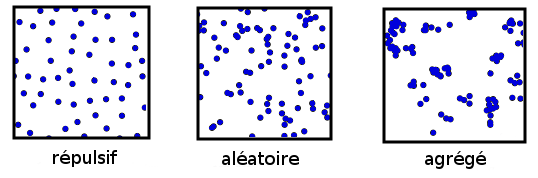
\includegraphics[scale=0.6]{figures/repartition2.png}
  \caption{Représentation des différentes formes de représentations spatiales de points}
  \label{fig:repartition}
\end{figure}

Une manière statistique de déterminer si une observation de points correspond à l'un ou l'autre de ces trois cas, est de mesurer sa déviance avec un \gls{PPPoiss}*, en effet ce type de \gls{PP}* à la propriété d'être totalement aléatoirement réparti.

%%%%%%%%%%%%

\section{L'indice de Ripley : fonction K}

\subsection{Principe}
Supposons qu'on se pose une question sur l'espacement entre les points dans un ensemble de points. Il serait alors naturel de regarder les distances entre chaque points. Si ces distances sont grandes, la répartition de point serait plutôt répulsive. Alors que si elles sont petites, la répartition de point serait plutôt agrégée.

\subsection{La fonction K empirique}
Soit \textbf{x} un \gls{PP}* sur une surface \begin{math} W \subseteq \mathbb{R}^2\end{math} \gls{stationnaire}* avec une intensité \begin{math}\lambda\end{math}. Les distances \begin{math} d_{ij} = ||x_i-x_j||\end{math} entre chaque point distinct \begin{math} x_i \end{math} et \begin{math} x_j \end{math} de l'ensemble \textbf{x} constituent une \gls{statDescriptive}*. Il est alors plus commode de travailler avec la fonction de distribution cumulative empirique donnée par:
\begin{align*}
\hat{H}(r) &= \text{taux des valeurs } d_{ij} \text{ plus petites que r } \\
        &= \frac{1}{n(n-1)} \sum_{i=1}^n \sum_{\underset{j \neq i}{j=1}}^n \mathds{1} \{d_{ij} \leq r \}
\end{align*}
défini pour chaque distance \begin{math} r \geq 0 \end{math}. La fonction indicatrice  \begin{math} \mathds{1} \{...\}\end{math} vaut 1 si son contenu est vrai et 0 sinon. La somme de ces indicatrices est simplement le nombre de fois où le contenu est vrai: le nombre de distance entre chaque point inférieur ou égal à r. Le dénominateur n(n-1) est le nombre total des paires de points distincts.

\begin{wrapfigure}{r}{7cm}
 \centering
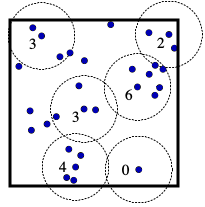
\includegraphics[width=6cm]{figures/nombreVoisins2.png}
\caption{Nombre de points voisin dans un certain rayon.}
\label{fig:nombreVoisins}

\end{wrapfigure} 

Comme le montre la figure~\ref{fig:nombreVoisins}, on cherche à estimer le nombre moyen de voisin dans un certain rayon r sur une certaine surface. Ainsi pour standardiser l'équation, il faut diviser l'expression par l'intensité \begin{math}\lambda \end{math} et pas seulement par (n-1). On peut alors faire un approximation de l'intensité sur la surface telle que: \begin{math}\lambda = (n-1)/|W|\end{math}.
Les points où le rayon dépassent du bord de la surface ne donneront pas des résultats exactes, il ne faut donc pas non plus négliger les effets de bords.

La fonction \begin{math}|W|\hat{H}(r)\end{math} est la moyenne standardisée du nombre de points voisins dans un rayon r pour un point type. Afin de prendre en compte les effets de bords, on ajoute une correction pour les effets de bords à \begin{math}\hat{H}\end{math}, ce qui nous donne la fonction K empirique:
\begin{align*}
\hat{K}(r) = \frac{|W|}{n(n-1)} \sum_{i=1}^n \sum_{\underset{j \neq i}{j=1}}^n \mathds{1} \{d_{ij} \leq r \} e_{ij}(r)
\end{align*}
où \begin{math}e_{ij}(r)\end{math} est une correction pour les effets de bords qui sera expliquée plus loin.\\

%%%%%%%%%%%%

\subsection{La fonction K pour un processus de Poisson stationnaire}

\begin{wrapfigure}[11]{r}{7.5cm}
\vspace{-0.8cm}
\begin{center}
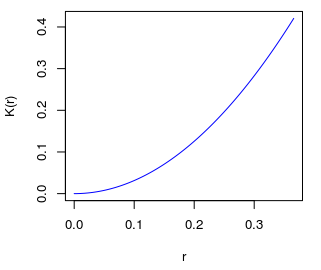
\includegraphics[width=6.5cm]{figures/Kpoiss2.png}
\caption{Représentation de la fonction K pour une répartition totalement aléatoire.}
\label{fig:Kpoiss}
\end{center}
\end{wrapfigure} 

En suivant la partie 7.3.2 du livre BaddEtal16~\cite{BaddEtal16}, on peut montrer que la fonction estimée par \begin{math}\hat{K}(r)\end{math} est donnée par:
\begin{align*} K_{pois}(r) = \pi r^2 \end{align*}
pour un processus de Poisson stationnaire d'intensité \begin{math}\lambda\end{math}

La figure~\ref{fig:nombreVoisins} montre alors la représentation en fonction de r de la fonction K théorique.

%%%%%%%%%%%%

\vspace{0.5cm}
\subsection{Interprétation de K}
La figure~\ref{fig:interpretK} ci dessous montre la fonction estimé de K selon si la configuration est agrégée aléatoire ou bien répulsive. Les courbes rouges représentent \begin{math}\hat{K}\end{math} tandis que les courbes bleues discontinues représentent \begin{math}K_{pois}\end{math}.\\

\begin{figure}[h]
  \centering
  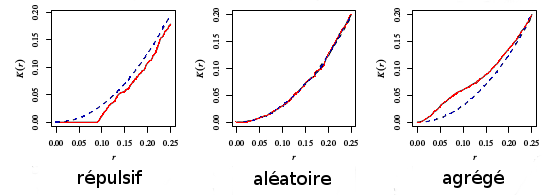
\includegraphics[scale=0.7]{figures/interpretK2.png}
  \caption{Différentes estimations de K.}
  \label{fig:interpretK}
\end{figure}


Sur la gauche, la courbe de la fonction calculée est en dessous de celle pour une répartition totalement aléatoire (\begin{math}\hat{K}(r) < K_{pois}(r) \end{math}). Ainsi, pour une distance r, un point quelconque a en moyenne moins de voisins qu'il aurait pu espérer avoir avec une répartition totalement aléatoire. Donc la répartition semble plutôt répulsive.\\
\indent
Sur la droite, la courbe de la fonction calculée est au dessus de celle pour une répartition totalement aléatoire (\begin{math}\hat{K}(r) > K_{pois}(r) \end{math}). Ainsi, pour une distance r, un point quelconque a en moyenne plus de voisins qu'il aurait pu espérer avoir avec une répartition totalement aléatoire. Donc la répartition semble plutôt agrégée.\\


%%%%%%%%%%%%%%%%%%%%%%%%%%%%%%%%%%%%%%%%%%%%%%%%%%%%%%%%%%%%%%%%
%%%%%%%%%%%%%%%%%%%%%%%%%%%%%%%%%%%%%%%%%%%%%%%%%%%%%%%%%%%%%%%%


\section{Fonction d'espace vide F}

\subsection{Définitions pour un processus de point stationnaire}
Si X est un processus ponctuel sur \begin{math} \mathbb{R}^2 \end{math}, la distance:
\begin{center}\begin{math} d(u,X) = min\{ ||u-x_i|| : x_i \in X \} \end{math}\end{center}
d'une position \begin{math} u \in \mathbb{R}^2 \end{math} au plus proche point d'un processus est appelé 'distance d'espace vide'.\\
Pour un processus de point stationnaire, la fonction de distance d'espace vide est:
\begin{center}\begin{math} F(r) = \mathbb{P}\{ d(u,X) \leq r \} \end{math}\end{center}
définie pour toute distance \begin{math} r \geq 0 \end{math}, où u est une position quelconque dans \begin{math} \mathbb{R}^2 \end{math}.\\

Les valeurs de F(r) sont les probabilités (valeur entre 0 et 1) pour n'importe quel position \textit{u} sur la surface, qu'il y ait un point x présent dans à une distance r ou moins de u (qu'il y ait un point dans le cercle de rayon r autour de u).\\

%%%%%%%%%%%%%%%%

\subsection{La fonction F pour un processus de Poisson stationnaire}

\begin{wrapfigure}[9]{r}{7.5cm}
\vspace{-0.8cm}
\begin{center}
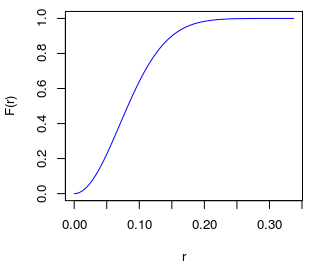
\includegraphics[width=6cm]{figures/poisson2.png}
\caption{Représentation de la fonction de répartition de Poisson.}
\label{fig:poisson}
\end{center}
\end{wrapfigure}

Pour un processus de Poisson stationnaire d'intensité \begin{math}\lambda\end{math}, on peut calculer:
\begin{align*}
F_{pois}(r) &= \mathbb{P}\{d(u,\textbf{x}) \leq r\} \\
            &= \mathbb{P}\{n( b(u,r) \cap \textbf{x} ) \neq 0\} \\
            &= 1 - \mathbb{P}\{ n( b(u,r) \cap \textbf{x} ) = 0\} \\
            &= 1 - exp(-\lambda \pi r^2)
\end{align*}
car par stationarité, F(r) ne dépend pas de u.\\
La figure~\ref{fig:poisson} montre la représentation en fonction de r de cette fonction théorique.\\


%%%%%%%%%%%%%%%%

\subsection{Estimation discrète de F}

Pour n'importe quelle position \textit{u} sur la surface à analyser, on mesure la distance \textit{d(u,\textbf{x})} la séparant du point voisin le plus proche (distance d'espace vide). On répète alors cette opération pour un nombre m de position \begin{math}u_1\end{math},...,\begin{math}u_m\end{math} équitablement réparties sur la surface. On peut alors calculer la fonction empirique:
\begin{align*} \hat{F}(r) = \frac{1}{m}\sum_{j=1}^m \mathds{1} \{d(u_j,\textbf{x}) \leq r \}\end{align*}
comme fonction sur la distance \begin{math} r \geq 0 \end{math}. Cependant, cette formule ne prend pas en compte les effets de bords, nous reviendrons plus loin sur ce point.

%%%%%%%%%%%%%%%%

\subsection*{Interprétation de F}
La figure~\ref{fig:interpretF} ci dessous montre la fonction estimé de F selon si la répartition est agrégée aléatoire ou bien répulsif. Les traits discontinues sont la représentation graphique de la fonction F théorique pour un aléatoire total.

\begin{figure}[h]
  \centering
  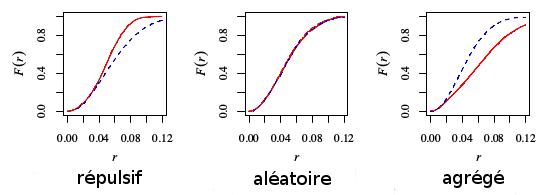
\includegraphics[scale=0.7]{figures/interpretF2.png}
  \caption{Différentes estimations de F.}
  \label{fig:interpretF}
\end{figure}

Sur la gauche, la courbe de la fonction calculée est au dessus de celle pour une répartition totalement aléatoire (\begin{math}\hat{F}(r) > F_{pois}(r) \end{math}). Ainsi, pour une distance r, la probabilité que \begin{math} d(u,X) \leq r \end{math} est plus grande quelle ne l'est pour une répartition aléatoire, les espaces vides sont donc plus petits que prévu. Donc la répartition semble plutôt répulsive.\\
\indent
Sur la droite, la courbe de la fonction calculée est en dessous de celle pour une répartition totalement aléatoire (\begin{math}\hat{F}(r) < F_{pois}(r) \end{math}). Ainsi, pour une distance r, la probabilité que \begin{math} d(u,X) \leq r \end{math} est plus petite quelle ne l'est pour une répartition aléatoire, les espaces vides sont donc plus grands que prévu. Donc la répartition semble plutôt agrégée.


%%%%%%%%%%%%%%%%%%%%%%%%%%%%%%%%%%%%%%%%%%%%%%%%%%%%%%%%%%%%%%%

\section{La fonction G pour un processus de Poisson stationnaire}

\subsection{Définitions pour un processus de point stationnaire}

Soit \begin{math}x_i\end{math} la réalisation d'un processus ponctuel \textbf{x}, la distance du plus proche voisin de  \begin{math}x_i\end{math} est écrite telle que:
\begin{center}\begin{math} d_i = d(x_i,\textbf{x}\backslash x_i ) \end{math}\end{center}
la plus courte distance de \begin{math} x_i \end{math} à un autre point de \textbf{x} excepté \begin{math} x_i \end{math}.
Pour un processus de point stationnaire X, la fonction de distance du plus proche voisin est:
\begin{center}\begin{math} G(r) = \mathbb{P}\{ d(u,X\backslash u) \leq r | u \in X \} \end{math}\end{center}
définie pour toute distance \begin{math} r \geq 0 \end{math}, où u est une position quelconque.\\

%%%%%%%%%%%%%%%%

\subsection{Valeurs pour un aléatoire complet}
Pour un processus de Poisson stationnaire  homogène d'intensité \begin{math}\lambda\end{math}, la fonction G est égale à la fonction d'espace vide F: 
\begin{center}\begin{math} G_{pois}(r) = 1 - exp(-\lambda \pi r^2) \end{math}\end{center}
Cela n'est vrai que pour une répartition totalement aléatoire, en général F et G seront des fonctions différentes.\\

%%%%%%%%%%%%%%%%

\subsection{Estimation discrète de G}

Pour un point \begin{math}x_i\end{math} de la configuration (\begin{math}\textbf{x} \cap B\end{math}), on mesure la distance \begin{math}d_i = d(x_i,\textbf{x}\end{math}\textbackslash\begin{math} x_i)\end{math} la séparant du point voisin le plus proche (distance du plus proche voisin). On répète alors cette opération pour tous les points \begin{math}x_1\end{math},...,\begin{math}x_n\end{math} de la configuration, avec n le nombre de point. On peut alors calculer la fonction empirique:
\begin{align*} \hat{G}(r) = \frac{1}{n}\sum_{i=1}^n \mathds{1} \{d_i \leq r \}\end{align*}
comme fonction sur la distance \begin{math} r \geq 0 \end{math}. Cependant, cette formule ne prend pas en compte les effets de bords, nous reviendrons plus loin sur ce point.

%%%%%%%%%%%%%%%%

\subsection{Interprétation de G }
La figure~\ref{fig:interpretG} ci-dessous montre la fonction estimée de G selon si la répartition est agrégée aléatoire ou bien répulsif. Les traits discontinus sont la représentation graphique de la fonction G théorique pour un aléatoire total.\\

\begin{figure}[h]
  \centering
  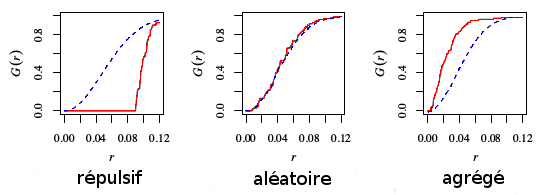
\includegraphics[scale=0.7]{figures/interpretG2.png}
  \caption{Différentes estimations de G.}
  \label{fig:interpretG}
\end{figure}

Sur la gauche, la courbe de la fonction calculée est en dessous de celle pour une répartition totalement aléatoire (\begin{math}\hat{G}(r) < G_{pois}(r) \end{math}). Ainsi, les distances des plus proches voisins sont plus grandes que celles prévues pour une répartition aléatoire. Donc la répartition semble plutôt répulsive.\\
\indent
Sur la droite, la courbe de la fonction calculée est au dessus de celle pour une répartition totalement aléatoire (\begin{math}\hat{G}(r) > G_{pois}(r) \end{math}). Ainsi, les distances des plus proches voisins sont plus petites que celles prévues pour une répartition aléatoire. Donc la répartition semble plutôt agrégée.\\


%%%%%%%%%%%%%%%%

\section{Fonction J}

Les distances du plus proche voisin et les distances d'espace-vide ont la même distribution de probabilité si la répartition des point est totalement aléatoire. Pour les départs des expériences avec une répartition aléatoire complète, ces distances ont tendance à répondre dans des directions opposées: l'un devient plus grand et l'autre plus petit. Cela suggère qu'une combinaison de ces 2 types de distance pourrait être utile pour évaluer les départs d'une répartition aléatoire.\\

Une combinaison pratique de G et F, suggérée par la théorie fondamentale, est la fonction J d'un processus stationnaire ponctuel:
\begin{center}\begin{math} J(r) = \frac{1-G(r)}{1-F(r)} \end{math}\end{center}
définie pour tout \begin{math} r \geq 0 \end{math} telle que F(r) < 1. Pour un processus de Poisson homogène, \begin{math} F_{pois} \equiv G_{pois} \end{math} ainsi les valeures de J(r) > 1 son cohérent avec une représentation répulsive, tandis que les valeurs de J(r) < 1 sont cohérente avec une représentation agrégée.


%%%%%%%%%%%%%%%%

\section{Correction des bords}

\subsection{Principe}

Une stratégie simple pour corriger les problèmes d'estimation sur les bords est la méthode de restriction des bords. Par exemple, lorsqu'on fait une estimation de K(r) pour une distance r, on limite les calculs aux point se trouvant à une distance r du bord de la surface étudiée. Ainsi le cercle de rayon r autour du point loge entièrement dans la surface comme le montre la figure~\ref{fig:bords}.

\begin{figure}[h]
  \centering
  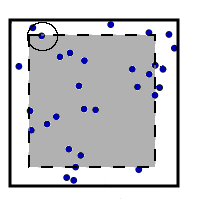
\includegraphics[scale=0.55]{figures/bords2.png}
  \caption{Exemple de zone de sûreté pour un certain rayon.}
  \label{fig:bords}
\end{figure}

%%%%%%%%%%%%%%%%

\subsection{Correction pour K}

En prenant en compte que les points dans la zone de sûreté pour chaque r, on peut alors réécrire \begin{math} \hat{K}(r) \end{math}. En gardant les mêmes notations qu'au 3.3.2 (La fonction K empirique), on peut écrire la fonction K avec correction des bords \begin{math} \hat{K}_{bord}(r) \end{math} telle que:
\begin{align*}
\hat{K}_{bord}(r) = \frac{  \sum_{i=1}^n \mathds{1} \{b_i \geq r \} \sum_{\underset{j \neq i}{j=1}}^n \mathds{1} \{d_{ij} \leq r \}}{\lambda \sum_{i=1}^n \mathds{1} \{b_i \geq r \}}
\end{align*}
où \begin{math}b_i\end{math} est la distance d'un point \begin{math}x_i\end{math} au bord de la surface, et \begin{math}\lambda\end{math} est l'estimation de l'intensité soit \begin{math}\lambda = n/|W|\end{math} avec |W| aire de la surface.

%%%%%%%%%%%%%%%%

\subsection{Correction pour F}

La même méthode de restriction des bords peut être appliquée à \begin{math} \hat{F}(r) \end{math}. Pour cette fonction, on ne se limite non pas aux points, mais aux positions \textit{u} qui sont à une distance du bord de la surface supérieur à r. Ainsi en gardant les mêmes notations qu'au 3.4.3 (Estimation discrète de F), on peut écrire la fonction F avec correction des bords:
\begin{align*}
\hat{F}_{bord}(r) = \frac{  \sum_{j=1}^m \mathds{1} \{d(u_j,\textbf{x}) \leq r \} \mathds{1} \{b_j > r \} }{ \sum_{j=1}^m \mathds{1} \{b_j > r \}}
\end{align*}
où \begin{math}b_j\end{math} est la distance d'une position \begin{math}u_j\end{math} au bord de la surface.

%%%%%%%%%%%%%%%%

\subsection{Correction pour G}

Pour appliquer la restriction des bords à \begin{math} \hat{G}(r) \end{math}, on se limite comme pour K aux points qui sont à une distance du bord de la surface supérieur à r. Ainsi en gardant les mêmes notations qu'au 3.5.3 (Estimation discrète de G), on peut écrire la fonction G avec correction des bords:
\begin{align*}
\hat{G}_{bord}(r) = \frac{  \sum_{i=1}^n \mathds{1} \{d_i \leq r \} \mathds{1} \{b_i \geq r \} }{ \sum_{i=1}^n \mathds{1} \{b_i \geq r \}}
\end{align*}
où \begin{math}b_i\end{math} est la distance d'un point au bord de la surface.

%%%%%%%%%%%%%%%%

\section{Test d'enveloppe}

On a vu dans les paragraphes précédents qu'il est possible d'interpréter les résultats des fonctions F,G,J et K en les comparant à la valeur quelles devraient avoir théoriquement pour une observation de point aléatoire. Cependant on ne peut pas tirer de conclusion précise. En effet une courbe correspondant exactement au cas Poissonien n'existe pas en pratique, une courbe qui est proche de celle théorique peut être considérée comme aléatoire. La question qui vient ensuite est celle de la limite: à partir de quel écart considère-t-on qu'une courbe cesse de représenter une répartition ponctuelle aléatoire? On peut alors se rendre compte des limites des informations fournies par de simple courbes. 

Un outil fournissant une meilleur estimation est le test d'enveloppe. Son principe est le suivant:
on lance les calculs des fonctions F, G, J et K sur un nombre n de configurations de points que l'on sait être aléatoires. On regarde ensuite les valeurs des n courbes obtenues. On peut tracer les courbes représentant les minimums et maximums atteints par les fonctions sur chaque abscisse. On obtient alors une enveloppe de toutes les valeurs obtenues pour les n courbes. 

\begin{figure}[h]
  \centering
  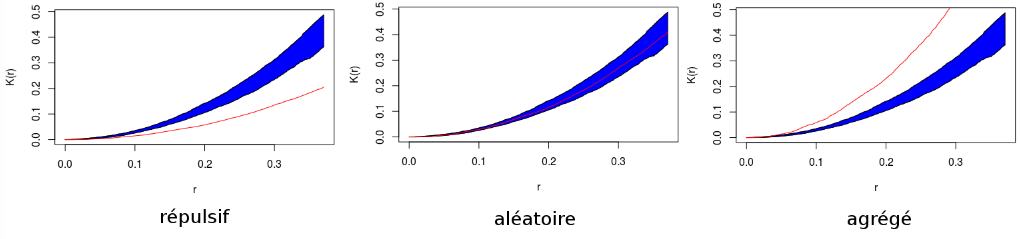
\includegraphics[scale=0.45]{figures/exempleEnveloppes.png}
  \caption{Exemple d'un test d'enveloppe sur la fonction K}
  \label{fig:enveloppeK}
\end{figure}

Ainsi s'il faut analyser une configuration, on peut maintenant comparer sa courbe avec l'enveloppe et faire une analyse plus précise de la répartition. Comme le montre le figure~\ref{fig:enveloppeK}, pour la fonction K: 
\begin{itemize}
\item si la courbe est en dessous de l'enveloppe, la répartition sera plutôt répulsive;
\item si la courbe est dans l'enveloppe, la répartition sera plutôt aléatoire;
\item si la courbe est au dessus de l'enveloppe, la répartition sera plutôt agrégée.\\
\end{itemize}

Remarque: Il n'est pas obligatoire de prendre le minimum et le maximum de chaque fonction pour faire l'enveloppe, on peut très bien faire par exemple un encadrement entre 2.5\% et 97.5\% pour éliminer les valeurs extrêmes.

%%%%%%%%%%%%%%%%

\newpage

%%%%%%%%%%%%%%%%%%%%%%%%%%%%%%%%%%%%%%%%%%%%%%%%%%%%%%%%%%%%%

\chapter{Réalisation}

\section{Environnement logiciel}

Une fois la théorie mathématique connue et comprise dans les grandes lignes, il fut possible de se mettre à l'implémentation. Le code du calcul a été écrit en C++ afin d'utiliser un langage compilé connu et utilisé par mon maître de stage et ainsi faciliter l'insertion de mon code dans ses programmes réalisés ultérieurement. De plus la partie graphique (affichage des courbes résultats) a été réalisé avec le logiciel R qui est très utilisé des statisticiens et qui possède une librairie "spatstat" dédiés aux calculs que je devais réaliser. Ainsi j'ai pu comparer mes résultats avec ceux de la librairie.\\

\section{Méthode de travail}

Tout au long du stage nous avons procédé étapes par étapes. En premier lieu, M. Radu Stoica me donnait des explications, puis me donnait de la documentation à lire sur la partie mathématique dans le livre BaddEtal16~\cite{BaddEtal16}. Ensuite après avoir lu et réfléchie sur une méthode de conception, je la partageais avec lui et nous en discutions. Il me proposait lui aussi des idées et nous regardions si elles pouvaient être inclue dans ma conception. De plus nous réfléchissions également pour savoir si nos méthodes étaient viable et rentable en terme de mémoire ou de temps d'exécution. Ensuite je réalisais le code. Une fois terminé, ou bien lorsque le travail était suffisamment avancé, je retournais voir M. Stoica pour faire le point. Nous regardions alors ce qui n'allait pas et ce qui pouvait être amélioré. Enfin je corrigeais les défauts de mon code et nous passions à une autre fonction en commençant par la partie théorique.\\

Ainsi j'ai eu à implémenter les fonctions K,G,F et J expliquées dans la partie 3 du rapport. Ensuite j'ai du prendre en main du code déjà écrit par M. Stoica afin d'insérer mes fonctions dedans. Il avait créé, à l'aide de 2 méthodes différentes, un générateur de répartitions ponctuels pouvant être plus ou moins aléatoire selon la modification des paramètres. Ainsi pour ses 2 méthodes, j'ai du itéré les opérations un certain nombre de fois et utiliser mes fonctions d'analyse sur les répartitions de points générés. On pouvait alors faire un test d'enveloppe qui permettra de mieux cerner le comportement de la répartition de points (explications partie 3 du rapport).\\

\newpage

%%%%%%%%%%%%%%%%
\section{Structure du code}

Pour réaliser les fonction j'avais à ma disposition des fichiers texte contenant les valeurs des positions (x,y) d'une répartition de point. De plus j'ai créé un fichier contenant des informations sur des paramètres expérimentaux que l'on pouvait donc modifié d'une expérience à l'autre. Ainsi j'avais 2 fichiers fournisseurs d'informations en entrée.
En analysant les calculs des fonctions, je me suis rendu compte que j'avais besoin de générer plusieurs information:
\begin{itemize}
\item la surface de la répartition;
\item un quadrillage sur toute la surface pour F;
\item les distances entre chaque points pour K et G;
\item les distances de chaque maille du quadrillage avec chaque points;
\item une liste d'abscisses de rayons.\\
\end{itemize}
Ainsi pour gérer le stockage de ces informations j'ai créé plusieurs classes. Une fois toutes la classes instanciées il a fallu les stocker, puis les traiter leur valeurs afin d'avoir le matériel nécessaire pour réaliser les calculs. Dans un soucis de présentation, je commencerai par présenter les objets nécessaire aux calculs, puis les algorithme des calculs, et enfin je parlerai de points plus précis du code. 

\subsection{Création des abscisses}

Pour les calculs des valeurs des fonctions, nous allons faire augmenter un rayon autour de chaque point ou maille. Ce seront les abscisses de nos fonction. On a appelle le derniers rayon, le rayon maximum: "rMAx".

Pour se rapprocher au maximum des courbes fournies par la \gls{spatstat}*, je suis aller chercher des informations sur la façon le code créé la liste des rayons (ses abscisses). J'ai alors trouvé sur site de spatstat\cite{FAQspatstat} qu'il fallait créer une liste de taille 513 (512 intervalles), les valeurs allant de 0 à Rmax.

Le calcul de Rmax est différent pour K et F,G,J. Ainsi j'ai trouvé qu'il fallait prendre le quart du plus petit des cotés du rectangle de surface comme rayon maximal pour la fonction K. Cependant, je n'ai rien trouver pour les autres fonctions.
J'ai donc fais une analyse de la situation: on a vu dans la partie 3 que pour une configuration aléatoire, les fonctions F et G sont définies par l'équation:
\begin{align*}
F_{poiss} = 1-exp(-\lambda.pi.r^2)
\end{align*}
Cette fonction tend vers 1, donc après un certain abscisse, les valeurs de la fonction seront toutes très proche de 1 et n'ajouteront plus d'information.
On cherche donc un rMax qui permettrait de ne garder que les valeurs inférieur à un gros pourcentage de la valeur finale de la fonction ( > à 90\%)
Alors en notant "P" le pourcentage de la valeur finale on peut écrire:
\begin{align*}
P = 1-exp(-\lambda.\pi.rMax^2)
\end{align*}
Une transformation rapide de l'équation permet d'exprimer clairement rMax en fonction de P:
\begin{align*}
rMax^2 = \frac{-ln(1-P)}{\pi.\lambda}
\end{align*}
Or en choisissant \begin{math}-ln(1-P)=\pi\end{math}:
\begin{align*}
P &= 1-exp(-pi)\\
&=0.9567
\end{align*}
Ainsi avec cette valeur de P on peut avoir un pourcentage de 96\% de la valeur finale tout en ayant un calcul simple de rMax:
\begin{align*}
rMax^2 = \frac{1}{\lambda}
\end{align*}
On a vu également Partie 3, que l'on peut calculer l'intensité lambda par le rapport du nombre de point n sur la taille de la surface W.

Ainsi prendre \begin{math} rMax^2 = \frac{W}{n} \end{math} permet de ne pas avoir de valeur infini mais de garder la majorité des informations importantes. 


\subsection{Les classes}

Comme le montre le diagramme de classe en Annexe~\ref{fig:diagClasse} j'ai créé 4 classes.

\subsubsection{La classe Rectangle}
Cette classe se veut être la représentation de la surface. Elle est défini par 4 valeur d'encadrement de type \gls{double}*:
\begin{itemize}
\item xMin défini par la plus petite valeur de x de la liste de point;
\item xMax défini par la plus grande valeur de x de la liste de point;
\item yMin défini par la plus petite valeur de y de la liste de point;
\item yMax défini par la plus grande valeur de y de la liste de point.\\
\end{itemize}

Ainsi cette classe permet de retourner l'aire total de la surface nécessaire pour le calcul de K avec un simple calcul:
\begin{lstlisting}[language=C++, caption={Méthode donnant l'aire de la surface}, label={lst:aireSurface}]
double Rectangle::getAire() const{
	return((xMax - xMin)*(yMax - yMin));
}
\end{lstlisting}
    
De plus cette classe permet de renvoyer la distance d'une position à la surface afin de gérer les effets de bord, pour des coordonnées (x,y):
\begin{lstlisting}[language=C++, caption={Méthode donnant la distance d'un point à la surface}, label={lst:distanceSurface}]
double Rectangle::distanceSurface(double x, double y) const{
	double d = xMax - x;
	if(d >= (x - xMin)){
		d = x - xMin;
	}
	if(d >= (yMax - y)){
		d = yMax - y;
	}
	if(d >= (y - yMin)){
		d = y - yMin;
	}
	return d;
}
\end{lstlisting}

\subsubsection{La classe Position}
Cette classe ne sera pas instanciée, elle servira de classe mère pour les classes Point et Quadrillage. Elle est définie par 2 coordonnées "x" et "y" de type \gls{double}* et une valeur de distance au bord de la surface "distanceBord" de type \gls{double}* également.\\

Les méthode de cette classe permettent d'accéder aux variables x,y et distanceBord.


\subsubsection{La classe Point}
Cette classe hérite de la classe Position, elle se veut être la représentation d'un point de la configuration d'entrée. En plus des caractéristiques de sa classe mère, elle possède la liste "listeDistancePoints" des distances la séparant de chacun des autres points de la configuration.

Cette classe permet alors de trier sa liste de distance de la plus petite à la plus grande afin de faciliter les calculs à venir, la méthode utilise le tri du \gls{namespace}* std qui sera expliquée plus en détail plus loin.
\begin{lstlisting}[language=C++, caption={Méthode triant la liste de distance}, label={lst:triListe}]
void Point::trierListe(){
	std::sort(listeDistancePoints.begin(), listeDistancePoints.end());
}
\end{lstlisting}

La classe permet également de recupérer un élément précis de sa liste de distance. Comme la liste aura été triée au préalable, plus on augmente l'indice en entrée de la méthode plus la valeur retourné sera grande :

\begin{lstlisting}[language=C++, caption={Méthode donnant le ième élément de la liste de distances}, label={lst:getDistanceDuPoint}]
double Point::getDistanceDuPoint(int i){
	return listeDistancePoints[i];
}
\end{lstlisting}


\subsubsection{La classe Quadrillage}
Cette classe hérite de la classe Position, elle se veut être la représentation d'une maille d'un quadrillage de la surface de la configuration de point. Elle sera utile pour le calcul de la fonction F. En plus des caractéristiques de sa classe mère, elle possède une valeur "distanceVide" de type \gls{double}* qui représente la distance la séparant du point de la configuration dont elle est le plus proche.

Cette classe contient ainsi une méthode permettant de trouver le point le plus proche et pour pouvoir initialiser sa variable:

\begin{lstlisting}[language=C++, caption={Méthode trouvant le point le plus proche d'une maille du Quadrillage}, label={lst:setDistanceVide}]
void Quadrillage::setDistanceVide(vector<Point> &point){
	
	int i=0;
	int n = (int)(point.size());
	double dX = 0;
	double dY = 0;
	double distance = 0;
	double dmin = 999999;

	for(i=0;i<n;i++){
		// calcul distances au carré
		dX = x - point[i].getX();
		dY = y - point[i].getY();

		distance = dX*dX + dY*dY;

		if(dmin > distance){
			dmin  = distance ;
		}
	}

	distanceVide = dmin;
}
\end{lstlisting}

La classe possède également une méthode permettant d'accéder à sa valeur de distance vide.

\subsection{Algorithmes globaux des fonctions}
Les algorithmes de calcul des fonction K et F,G,J sont représentés en Annexe~\ref{lst:algoFGJ}. On suppose qu'on a préalablement rangé et trié les valeur de distance à comparer.

Pour K, on procède point par point: on calcule combien chaque point a de voisin pour chaque rayon. Si un point est trop près du bord par rapport à la taille d'un rayon, on n'ajoute pas son nombre de voisin. La liste des point étant préalablement trié par rapport à leur distance au bord, on peut arrêter la boucle sur les points dès qu'un Point n'est plus dans la zone de sûreté.\\
De même en ayant trié les distances entre les points, on peut arrêter la boucle sur les distances aux autres points dès qu'une distance dépasse la valeur de rayon. On peut alors garder la valeur du nombre de voisin, et reprendre le calcul pour rayon suivant plus grand.
En effet, comme les listes ont étés préalablement triés, une fois la valeur de rayon dépassée toutes les valeurs suivantes seront 

Pour F,G et J, on procède point par rayon: pour chaque rayon, on calcul la valeur de F et de G puis on en déduit la valeur de J. Ainsi on compare la valeur de chaque rayon avec les valeurs de distance du plus proche voisin de : chaque point pour G et de chaque quadrillage pour F. De plus comme pour K, en triant les liste de Point et de Quadrillage en fonction de leur distance au bord, on peut optimiser les calculs de correction d'effet de bord.

\subsection{Les Listes}

Présente à plusieurs endroit du code, l'objet Vector du \gls{namespace}* std m'a été très utile. En effet, c'est ce type de liste que j'ai utilisé pour:
\begin{itemize}
\item la liste de Point;
\item la liste de Quadrillage;
\item chaque liste de distance dans les objets Points;\\
\end{itemize}

Comme on peut le voir sur le site cppreference.com\cite{vector} std::vector est un conteneur séquentiel qui encapsule les tableaux de taille dynamique.

Comme les tableaux, l'objet vector utilise un stockage contigüe, ce qui signifie que les éléments sont accessibles non seulement via les itérateurs, mais aussi à partir des pointeurs classiques sur un élément. A la différence des tableaux, la taille du vecteur peut être modifiée dynamiquement, c'est à dire que son stockage est pris en charge automatiquement, pouvant être augmenté ou diminué au besoin.

La complexité des opérations courante sur les vector sont les suivantes :
\begin{itemize}
\item Accès aléatoire - constante O(1);
\item Insertion ou le retrait d'éléments à la fin - constante amortie O(1);
\item Insertion ou le retrait d'éléments - linéaire O(n);\\
\end{itemize}

Au vu du nombre important d'accès aux valeurs des listes pour les calcul, le choix de cette structure m'a paru adapté.

\subsection{Les tris}

On peut se demander pourquoi avoir choisi de travailler sur des liste plutôt que sur des matrices pour gérer les distances entre chaque point et le quadrillage. C'est là qu'intervient le tri. En effet en triant les listes précédemment définies on peut éviter de nombreux calculs.

Il a ainsi fallu classer les listes de Point et de Quadrillage de l'objet le plus éloigné du bords au plus proche pour les deux listes. De plus pour chaque objet Point il a fallu trier la liste de distance aux autres point de la plus petite à la plus grande.

La méthode de tri utilisée fut la méthode "sort" du \gls{namespace}* std. Selon le site cppreference.com\cite{sort} std::sort est un tri optimisé qui utilise l'algorithme de tri "introsort" hybride entre le tri rapide et tri par tas. Il fourni ainsi une vitesse de calcul rapide pour le cas moyen, et des performances optimales dans le pire des cas. Ce tri possède ainsi une complexité de \begin{math}n.log(n)\end{math} dans tous les cas.

L'étude\cite{PerfSort} mené par une élève de l'ISIMA, à Clermont-Ferrand montre les avantages l'efficacité de std::sort sur l'objet std::vector.


%%%%%%%%%%%%%%%%

\section{Astuces}

%Afin d'accéléré les temps de calculs j'ai mis en place différentes astuces de code.

\subsection{Le remplissage des listes de distance}
Comme chaque point possède la liste des distance aux autres points, on peut se représenter le tableau suivant:\\
\hspace*{3cm}
\begin{tabular}{c|cccccc}
   & point 1 & point 2 & ... & point j & ... & point n \\
  \hline
  point 1 & 0 & \begin{math} d_{12} \end{math} & ... & \begin{math} d_{1j} \end{math} & ... & \begin{math} d_{1n} \end{math} \\
  point 2 & \begin{math} d_{21} \end{math} & 0 & ... & \begin{math} d_{2j} \end{math} & ... & \begin{math} d_{2n} \end{math}\\
  ... & ... & ... &  ...  & ... & ... & ... \\
  point i & 0 & \begin{math} d_{i2} \end{math} & ... & \begin{math} d_{ij} \end{math} & ... & \begin{math} d_{in} \end{math} \\
   ... & ... & ... & ... & ... & ... & ... \\
  point n & \begin{math} d_{n1} \end{math} & \begin{math} d_{n2} \end{math} & ... & \begin{math} d_{nj} \end{math} & ... & 0 \\
\end{tabular}

Or la distance d'un point i à un point j est la même que celle d'un point j à un point i, c'est à dire que \begin{math} d_{ij} = d_{ji}\end{math}. On n'a besoin de ne calculer que la partie triangulère supérieure du tableau pour avoir toutes les valeurs.\\

\begin{lstlisting}[language=C++, caption={Remplissage des listes de distance}, label={lst:distances}]
int i;
int j;
double dX = 0;
double dY = 0;
double distance = 0;

for( i = 1; i < n-1; i++){
    for( j = i; j < n; j++){
        dX = point[j].getX() - point[i].getX();
		dY = point[j].getY() - point[i].getY();

 		distance  = dX*dX + dY*dY ;
 		
 		point[i].ajoutDistance( distance );
        point[j].ajoutDistance( distance );
    }
}
\end{lstlisting}

Ainsi en applicant la méthode ci dessus, on peut faire moitié moins d'opérations: pour n points, on économise n(n-1)/2 opérations.

\subsection{Les distances aux carrés}

La majorité des calculs concernent des calculs de distance. Ainsi entre 2 points A et B d'abscisses et d'ordonnées respectives (xA,yA) et (xB,yB) la distance ce calcul par la formule de Pythagore:
\begin{align*}
distance = \sqrt{(xB-xA)^2 + (yB-yA)^2}
\end{align*}
Or le calcul de la racine carrée prend du temps et peut être évité.\\

En effet, ces distance vont être par la suite seulement comparées, ainsi pour un rayon "r" et une distance entre 2 points "d":
\begin{align*}
d < r  \Leftrightarrow  d^2 < r^2
\end{align*}
Ainsi, il est utile de ne stocker que les valeurs au carré des calculs de distance. En notant ts le temps de calcul d'une racine carrée, on gagne:

\hspace*{1cm} t = (n*(n-1)/2)*ts \hspace*{1cm} pour les calculs de distance point/point

\hspace*{1cm} t = (m*n)*ts \hspace*{1cm} pour les calculs de distance maille/point\\

\subsection{Arrêter les calculs et stockage au rayon maximal}
Pour le calcul de K, pour chaque point on incrémente un compteur selon le nombre de voisin qu'a le point étudié dans un certain rayon. Tous les points à une distance plus grande que le plus grand rayon rMax ne seront donc jamais pris en compte. Ainsi lors du remplissage des listes de distance, il est inutile de stocker les distances entre 2 points éloigné de plus de rMax. Cela permet d'economiser beacoup de mémoire, mais aussi de réduire drastiquement le temps de calcul:  moins de temps d'ajout dans les listes, des tris plus rapides et moins de calcul à la fin.

\section{Tests d'enveloppe}

à faire

il faudrait que je demande des précisions sur "araint" et "strauss"

\newpage

%%%%%%%%%%%%%%%%%%%%%%%%%%%%%%%%%%%%%%%%%%%%%%%%%%%%%%%%%%%%%

\chapter{Bilan}

\section{Résultats obtenus}

\subsection{Validation}

Une fois les fonction réalisées, il a fallu s'assurer que les résultats étaient bon, que les fonctions ne font pas d'erreur de calcul. Pour cela j'ai pu m'aider de la \gls{spatstat}* pour comparer les courbes obtenues avec mes calculs avec celles réalisées par leurs algorithmes.

Comme on peut le voir en Annexe~\ref{fig:compSpatstat} le résultat final colle bien aux attentes. Il est difficile de distinguer à l'oeil les écarts entre les courbes, sauf pour la fonction J pour laquelle la différence est engendrée par de petits écarts sur les fonctions F et G.
Lorsqu'on compare les valeurs précises prises par les fonctions, on trouve des écarts de ordre de:
\begin{itemize}
\item \begin{math}10^{-4}\end{math} pour K,
\item \begin{math}10^{-7}\end{math} pour G,
\item \begin{math}10^{-3}\end{math} pour F.\\
\end{itemize}

Les écart sont raisonnables, on peut donc considérer les calculs de fonction valides.

%%%%%%%%%%%%%%%%%%%%%%%%%

\subsection{Visualisation}

Les codes en C++ écrivent des valeurs dans un fichier texte, ces valeurs sont ensuite lues par un programme R qui traite alors les résultats. Ensuite une fois les résultats rapidement analysés (recherche des minimums et maximums pour le test d'enveloppe), ce même programme affiche les courbes résultantes des valeurs calculées par le premier programme.

En Annexe~\ref{fig:compPoisson} sont représentés les résultats des calculs des fonctions F,G,J et K avec leur courbes d'aléatoire respective pour une observation. Ainsi on peut constater que cette distribution est un peu plus répulsive que ne le serait une distribution complètement aléatoire.

En Annexe~\ref{fig:testEnveloppe} est représenté le résultat des test d'enveloppe. La dernière courbe analysée y est représentée également en tant qu'exemple.

\newpage

%%%%%%%%%%%%%%%%%%%%%%%%%

\subsection{Utilisation}

Vous pouvez trouver le projet en libre accès sur github, à l'adresse:\\
\hspace*{2cm} \url{https://github.com/DugueC/Stage2A}\\

Les codes fonctionnent à condition d'avoir installer un compilateur c++ et R.\\
Si un script ne fonctionne pas, essayer de donner les droits au fichier\\ ( chmod 777 nom\_script.sh ).
 
%%%%%%%%%

\subsubsection{Dossier calculFGJK}

Ce dossier contient la partie de calcul de fonction uniquement

Pour compiler:
\begin{itemize}[label=\textbullet]
\item ./make main\\
\end{itemize}

Pour lancer le code:
\begin{itemize}[label=\textbullet]
\item mettre un fichier avec la liste des points dans le dossier "POINTS"
\item changer les paramètres au besoin dans le dossier "PARAMS"
\item au choix:
    \begin{itemize}[label=\textbullet]
    \item ./calcul
    \item  ./visualisation.sh - si vous voulez afficher les courbes également\\
    \end{itemize}
\end{itemize}



%%%%%%%%%

\subsubsection{Dossier codeComplet}

Ce dossier contient le code permettant de faire la génération des tests d'enveloppe.

Pour compiler, selon le type de génération recherchée:
\begin{itemize}[label=\textbullet]
\item aller dans le dossier "STRAUSS"
\item ./make \\
OU
\item aller dans le dossier "AREAINT"
\item ./make
\end{itemize}

Pour lancer le code:
\begin{itemize}[label=\textbullet]
\item changer les paramètres au besoin dans le dossier "PARAMS"
\item aller dans le dossier "EXEC"
\item au choix:
    \begin{itemize}[label=\textbullet]
    \item ./sim\_cftp.exe ../PARAMS/nom\_param.txt
    \item ./sim\_areaint.exe ../PARAMS/nom\_param.txt
    \item ./enveloppes\_sim\_cftp.sh ../PARAMS/nom\_param.txt
    \item ./enveloppes\_sim\_areaint.sh ../PARAMS/nom\_param.txt
    \end{itemize}
\end{itemize}

Les 2 scripts permettent d'avoir une visualisation juste après les calculs.


%%%%%%%%%%%%%%%%%%%%%%%%%

\section{Difficultés rencontrées}

Les premières difficultés sont intervenues dès le début du stage. N'étant pas à l'aise avec le langage C++, et ne connaissant pas le langage R, j'ai mis un certain temps à m'adapter et me documenter. J'ai également parfois demandé de l'aide pour mes affichages de fonction réalisé en R, tâche pourtant basique. La barrière du langage à donc freiné dans un premier temps l'avancée du projet.

Une fois les fonctions réalisées en procédant simplement par un suivi intuitif des équation des fonctions théoriques, il a fallu accéléré les temps calculs. En effet mon programme n'était pas optimisé dans une optique de gain de temps et n'était donc pas très performantes dès que les configurations de points étaient trop fournies. J'ai donc revu mes algorithmes et trouvés des astuces afin que le temps de calcul des fonctions soit du même ordre que celui réalisé par la \gls{spatstat}*. Cela n'a pas toujours été facile notamment pour les changements d'algorithmes.

%%%%%%%%%%%%%%%%%%%%%%%%%

\section{Suite du projet}

\subsection{Développements futurs}
L'ensemble du projet a été réalisé en 2 dimensions, c'est à dire que les points fournies n'avaient que deux coordonnées spatiales. Une adaptation du code pour une 3ème dimension ouvrirait la porte à un nouveau panel d'expériences qu'il serait possible d'analyser.

Mon maître de stage M. Radu Stoica fait d'ailleurs en se moment e  d'ailleurs sur la façon dont sont réparties des regroupement de sel dans un marais salant. Les particules salées ne sont alors pas seulement réparties sur un plan horizontale, mais dans un volume d'eau.

%%%%%%%%%%%%%%%%%%%%%%%%%

\subsection{Devenir du projet}
M. Stoica pourra utiliser ces programmes pour faire des expériences ... demander à Radu ce qu'il veut faire précisément avec le projet

%%%%%%%%%%%%%%%%%%%%%%%%%%%%%%%%%%%%%%%%%%%%%%%%%%%%%%%%%%%%%

\chapter{Conclusion}


%L'objectif de ce stage à été atteint: les outils informatiques pour traiter les données ponctuels ont été réalisés (fonctions F,G,J et K) et intégrés au code de mon maître de stage afin d'analyser ces données (test d'eveloppe).

%un bilan : leçons théoriques et pratiques à partir des résultats et à partir de l'expérience au sein de l'entreprise ;  

%une  ouverture  :  réalisations  qui  peuvent  être  envisagées  à  partir  des  résultats  obtenus / confirmation du projet professionnel...

%Finalement cette expérience m'a fait découvrir un monde de la recherche en mathématique et un nouveau mode de travail ...  


\newpage
~
\newpage

%%%%%%%%%%%%%%%%%%%%%%%%%%%%%%%%%%%%%%%%%%%%%%%%%%%%%%%%%%%%%


\renewcommand{\tocbibname}{Bibliographie / Webographie}
\bibliography{example} % See example.bib 
\bibliographystyle{plain}



%%% liste des illustrations
\listoffigures
\newpage

%%% liste de tableaux
%\listoftables
%\newpage

\lstlistoflistings
\newpage


%%% Glossaire
%\chapter*{Glossaire}
\printglossaries
\addcontentsline{toc}{chapter}{Glossaire}

\newpage
~
\newpage

\appendix
\part*{Annexes}
\addcontentsline{toc}{part}{Annexes}
\newpage

\chapter{Diagramme de Classes}
\begin{figure}[h]
  \centering
  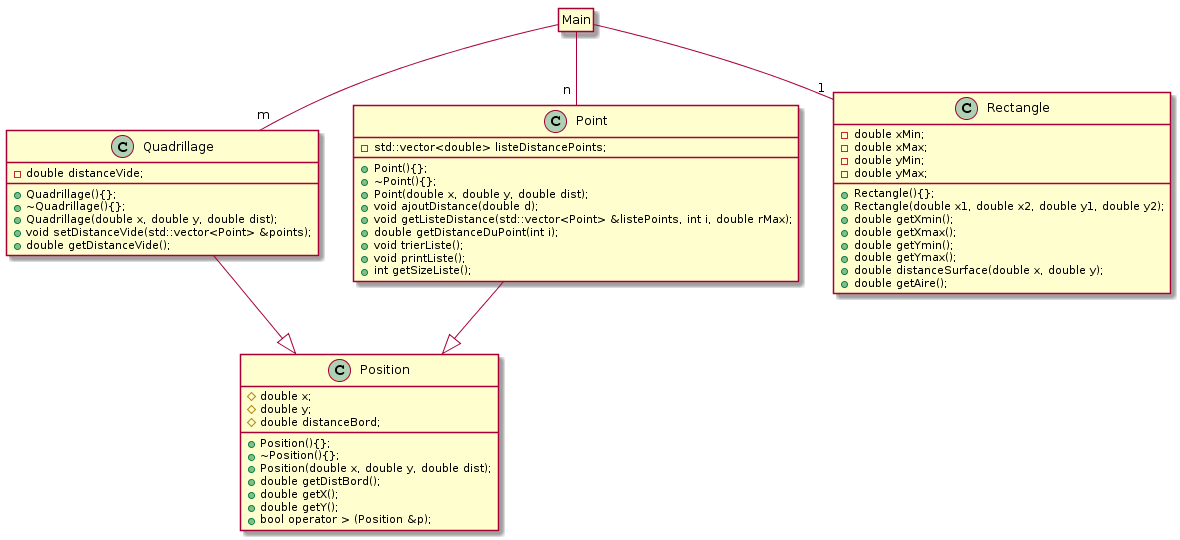
\includegraphics[scale=0.45]{figures/diagrammeClasses.png}
  \caption{Diagramme de classe pour les calculs des fonctions}
  \label{fig:diagClasse}
\end{figure}
\newpage


\chapter{Algorithmes des calculs des fonctions}
\lstset{
    keywordstyle=\bfseries,
    morekeywords={ ENTREE, CONSTANTES, LISTES, POUR, TANT, QUE, INCREMENTER, ET, SAUVEGARDER, VARIABLES, SI, SINON},
}

\begin{lstlisting}[ caption={Algorithme fonction K}, label={lst:algoK}]
ENTREE : Liste de Points

CONSTANTES :
    n = nombre de points dans liste
    nR = nombre de rayons à analyser
    aire = aire de la surface couverte par les points de la liste

LISTES : 
    NombrePointsConsideres[]
    Kcumule[]
    
VARIABLES :
    i = 0
    j = 0
    k = 0

POUR ( i de 0 à n )
{
    j = 0
    
    TANT QUE ( distance du point i au bord  >  au j-eme rayon )
          ET ( j < nR )
    {
        INCREMENTER NombrePointsConsideres[j]
         
        TANT QUE ( distance du point i au point k < j-eme rayon)
              ET ( k < n - 1 )
        {
            INCREMENTER k
        }
        
        Kcumule[j] = Kcumule[j] + k
        
        INCREMENTER j
    } 
}
    
POUR ( j de O à nR )
{
		SAUVEGARDER K[j] = Kcumule[j]*aire/((n-1)*NombrePointsConsideres[j])
}

\end{lstlisting}

\newpage

\begin{lstlisting}[ caption={Algorithme fonction F, G et J}, label={lst:algoFGJ}]
ENTREE : Liste de Points

CONSTANTES :
    nP = nombre de points dans liste
    nQ = nombre de quadrillage
    nR = nombre de rayons à analyser
    aire = aire de la surface couverte par les points de la liste

VARIABLES :
    i = 0
    j = 0
    k = 0
    sommeF = 0
    sommeG = 0

POUR ( k de 0 à nR )
{
    i = 0
    
    TANT QUE ( distance du point i au bord  >=  au k-eme rayon )
          ET ( i < nP )
    {
        SI ( distance du point i au plus proche point voisin <= k-eme rayon)
        {
            INCREMENTER sommeG
        }
        INCREMENTER i
    }
    
    j = 0
    
    TANT QUE ( distance du quadrillage j au bord  >  au k-eme rayon )
          ET ( j < nQ )
    {
        SI ( distance du quadrillage j au plus proche point voisin <= k-eme rayon)
        {
            INCREMENTER sommeF
        }
        INCREMENTER j
    }
    
    SAUVEGARDER G = sommeG/i
    SAUVEGARDER F = sommeF/j
    
    SI ( F==1 )
    {
        SAUVEGARDER J = INFINI
    }
    SINON
    {
        SAUVEGARDER G = (1-G)/(1-F)
    }
}
\end{lstlisting}

\newpage


\chapter{Représentations sous R}

\begin{center}
\begin{figure}[h]
  \centering
  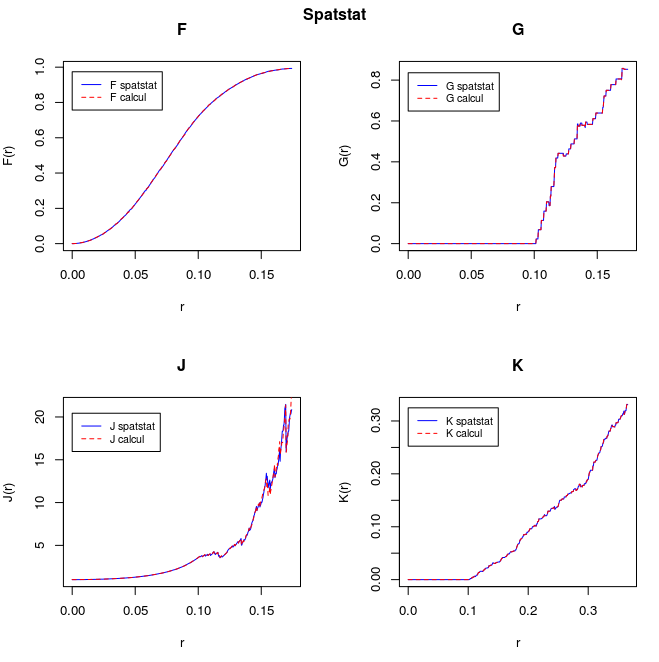
\includegraphics[scale=0.7]{figures/calcul&spatstat.png}
  \caption{Comparaison des fonctions programmées avec celles calculées par spatstat }
  \label{fig:compSpatstat}
\end{figure}
\end{center}
\newpage

\vspace*{2cm}
\begin{center}
\begin{figure}[h]
  \centering
  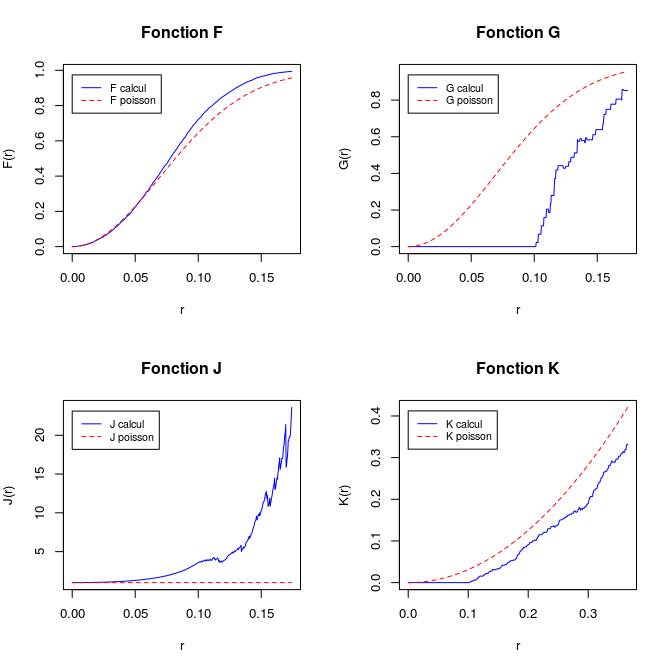
\includegraphics[scale=0.7]{figures/calcul&poisson.png}
  \caption{Comparaison des fonctions programmées avec courbes théoriques pour une répartition aléatoire}
  \label{fig:compPoisson}
\end{figure}
\end{center}
\newpage

\vspace*{2cm}
\begin{center}
\begin{figure}[h]
  \centering
  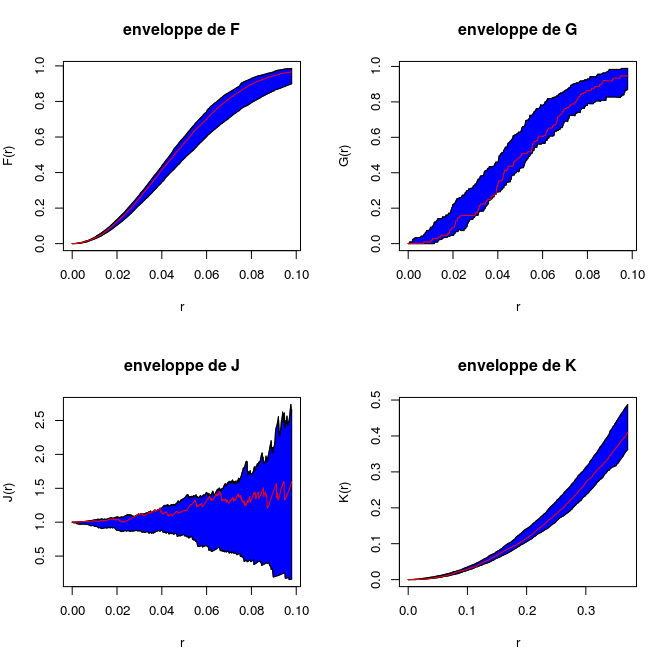
\includegraphics[scale=0.7]{figures/calculEnveloppes.png}
  \caption{Exemple de résultat des tests d'enveloppes}
  \label{fig:testEnveloppe}
\end{figure}
\end{center}
\newpage
~
\newpage

\thispagestyle{empty}

\section*{Résumé}
\addcontentsline{toc}{chapter}{Résumé}

Ce rapport présente le travail de stagiaire effectué dans l'équipe Probabilité-Statistique de l'Institut Elie Cartan de Lorraine. Ce projet s'inscrit dans le cadre d'un stage de 2ème année à TELECOM Nancy. Le stage a pour but la création d'outils informatique pour traiter et analyser des données ponctuelles selon des méthodes mathématiques d'analyse statistique. Les fonctions à modéliser visent à estimer si les points d'une représentation sont plus ou moins répartis aléatoirement.\\

Avec une génération de répartitions ponctuels créé par M. Radu Stoica, il est possible de faire une enveloppe de valeurs qui permet d'avoir une estimation plus précise de la tendance de répartition des points. Ainsi, les résultat de ce projet permettrons à M. Stoica de faire de futurs analyses de situations plus précises.\\

{\bf Mots-clés : analyse statistique, analyse,processus ponctuel }


\section*{Abstract}
\addcontentsline{toc}{chapter}{Abstract}

This report present a trainee work for the Probability-Statistique team of the "Institut Elie Cartan de Lorraine". This project was realised in the framework of a 2nd year trainee in TELECOM Nancy. The goal of the traineeship is to create an computer tool in order to treat and analyze data point with statistical method. The functions to develop intend to estimate the ramdom degree of a point pattern.

With a point pattern generator created by Mr Radu Stoica, it is possible to make a data envelop which allow a more precise estimation of the point repartition trend. Thus, the results of this project would allow Mr Stoica to carry out  more precise analysis in the futur.

{\bf Keywords : statistic, analysis point process}

\end{document}